\chapter{Effects of hydrodynamic interactions on the dispersion of Brownian solutes in fluid flows}
\label{ch:4}


\section{Introduction}
Fluid flows are ubiquitous in many biological settings. The study of fluid dynamics provides insights on multiple ranges of applications.
Oceanic currents and large-scale weather phenomena ~\cite{pedlosky_geophysical_1987}, the lift of an airplane foil ~\cite{anderson_aerodynamics_2016}, surfing ~\cite{butt_physics_2024} and drug delivery all rely at least partly on fluid dynamics. The latter example is particularly relevant to my thesis, as it is a perfect example of the interplay between a fluid flow and Brownian motion for the diffusive transport of drugs in the bloodstream. In this chapter, I focus on the study of Brownian motion in fluid flows, and more specifically in viscous flows, with dense suspensions and hydrodynamic interactions as a main problem. 

\subsection{The Reynolds number}
We commonly use the Reynolds number $\mathrm{Re}$ o evaluate the relative importance of inertial effects in a fluid over viscous ones. It reads:
\begin{equation}
    \mathrm{Re} = \dfrac{\rho U L}{\eta}~,
    \label{Reynolds_number}
\end{equation}
where $\rho$ is the fluid's density, $U$ is a characteristic velocity, $L$ is a characteristic length and $\eta$ is the fluid's dynamic viscosity. Turbulence in a flow occurs at high Reynolds number, \emph{i.e.} $\mathrm{Re} \gg \, 1$, whereas a fluid flow with small Reynolds number $\mathrm{Re}\ll \, 1 $ is considered laminar, with a layered and constant profile. A classic example is that of cigarette smoke (Fig.~\ref{ciggy}). The smoke exits the cigarette's tip at low velocity. By taking air density at room temperature $\rho_\mathrm{air} = 1.2 \, \mathrm{kg}.\mathrm{m}^{-3}$, viscosity at about $\eta_\mathrm{air} = 1.8\times 10^{-5}\, \mathrm{Pa.s}$, and a smoke characteristic velocity $U_\mathrm{smoke} = 1 \,\mathrm{cm}.\mathrm{s}^{-1}$ and characteristic plume width $L_\mathrm{smoke} = 1 \, \mathrm{mm}$, the first regime has $\mathrm{Re} = 0.5\,$. Higher up, the smoke rises much faster and the plume is wider, with a characteristic speed of $U_\mathrm{smoke} = 10 \, \mathrm{cm}.\mathrm{s}^{-1}$ and a characteristic width of about $L_\mathrm{smoke} = 2 \, \mathrm{cm}$, the ratio gives $\mathrm{Re} \approx \,100$. Perturbations are suppressed in the first regime due to viscous effects. As the speed rises, perturbations can no longer be damped, and the typical turbulences arise.


\begin{figure}
    \centering
    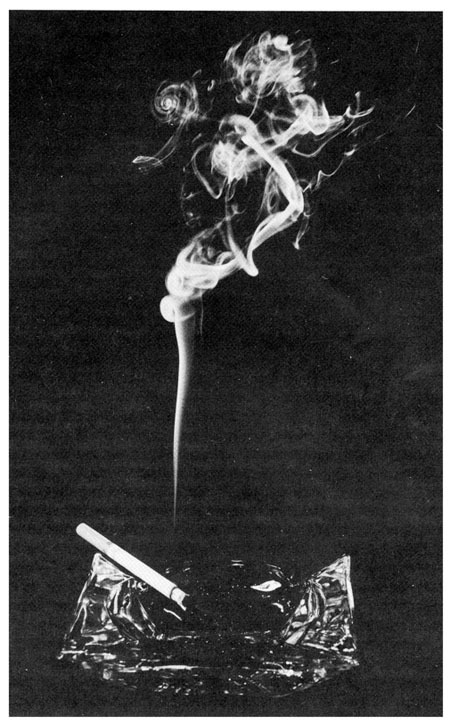
\includegraphics[width=0.3\textwidth]{figures/chapter4/ciggy.jpg}
    \caption[Illustration of the laminar and turbulent regimes with cigarette smoke.]{Smoke rising from a lit cigarette tip. At short distances from the tip, the smoke plume is narrow and the velocity low enough for the flow to be considered laminar. Higher up, the plume is wider and the velocity higher; the flow transitions to a turbulent one. Source: Physics Stack Exchange.}
    \label{ciggy}
\end{figure}
Most microfluidic experiments and associated simulations are conducted in the low-Reynolds-number regime. Despite the apparent simplicity of Stokes flows, this regime exhibits a wide range of rich phenomena, including non-trivial transport, mixing, particle migration, and microswimmer dynamics ~\cite{purcell_life_1977, squires_microfluidics_2005}. In the framework of this thesis, I am interested in understanding the coupling between hydrodynamically interacting colloids, fluid flows and confinement. Specifically, one question has already been well investigated in the last century: \emph``W{hat happens to a Brownian solute once it is advected by a low-Reynolds, viscous flow?''} In this chapter, I first introduce the classical Taylor-Aris theory, developed to predict the dispersion of a Brownian solute under advection. Then, I present the results of a collaboration with Joshua McGraw, Masoodah Gunny, Alexandre Vilquin, Blaise Delmotte and Elodie Millan, investigating hydrodynamic interactions in a Brownian solute under flow advection. 


\subsection{Taylor-Aris dispersion}
\begin{figure}
    \centering
    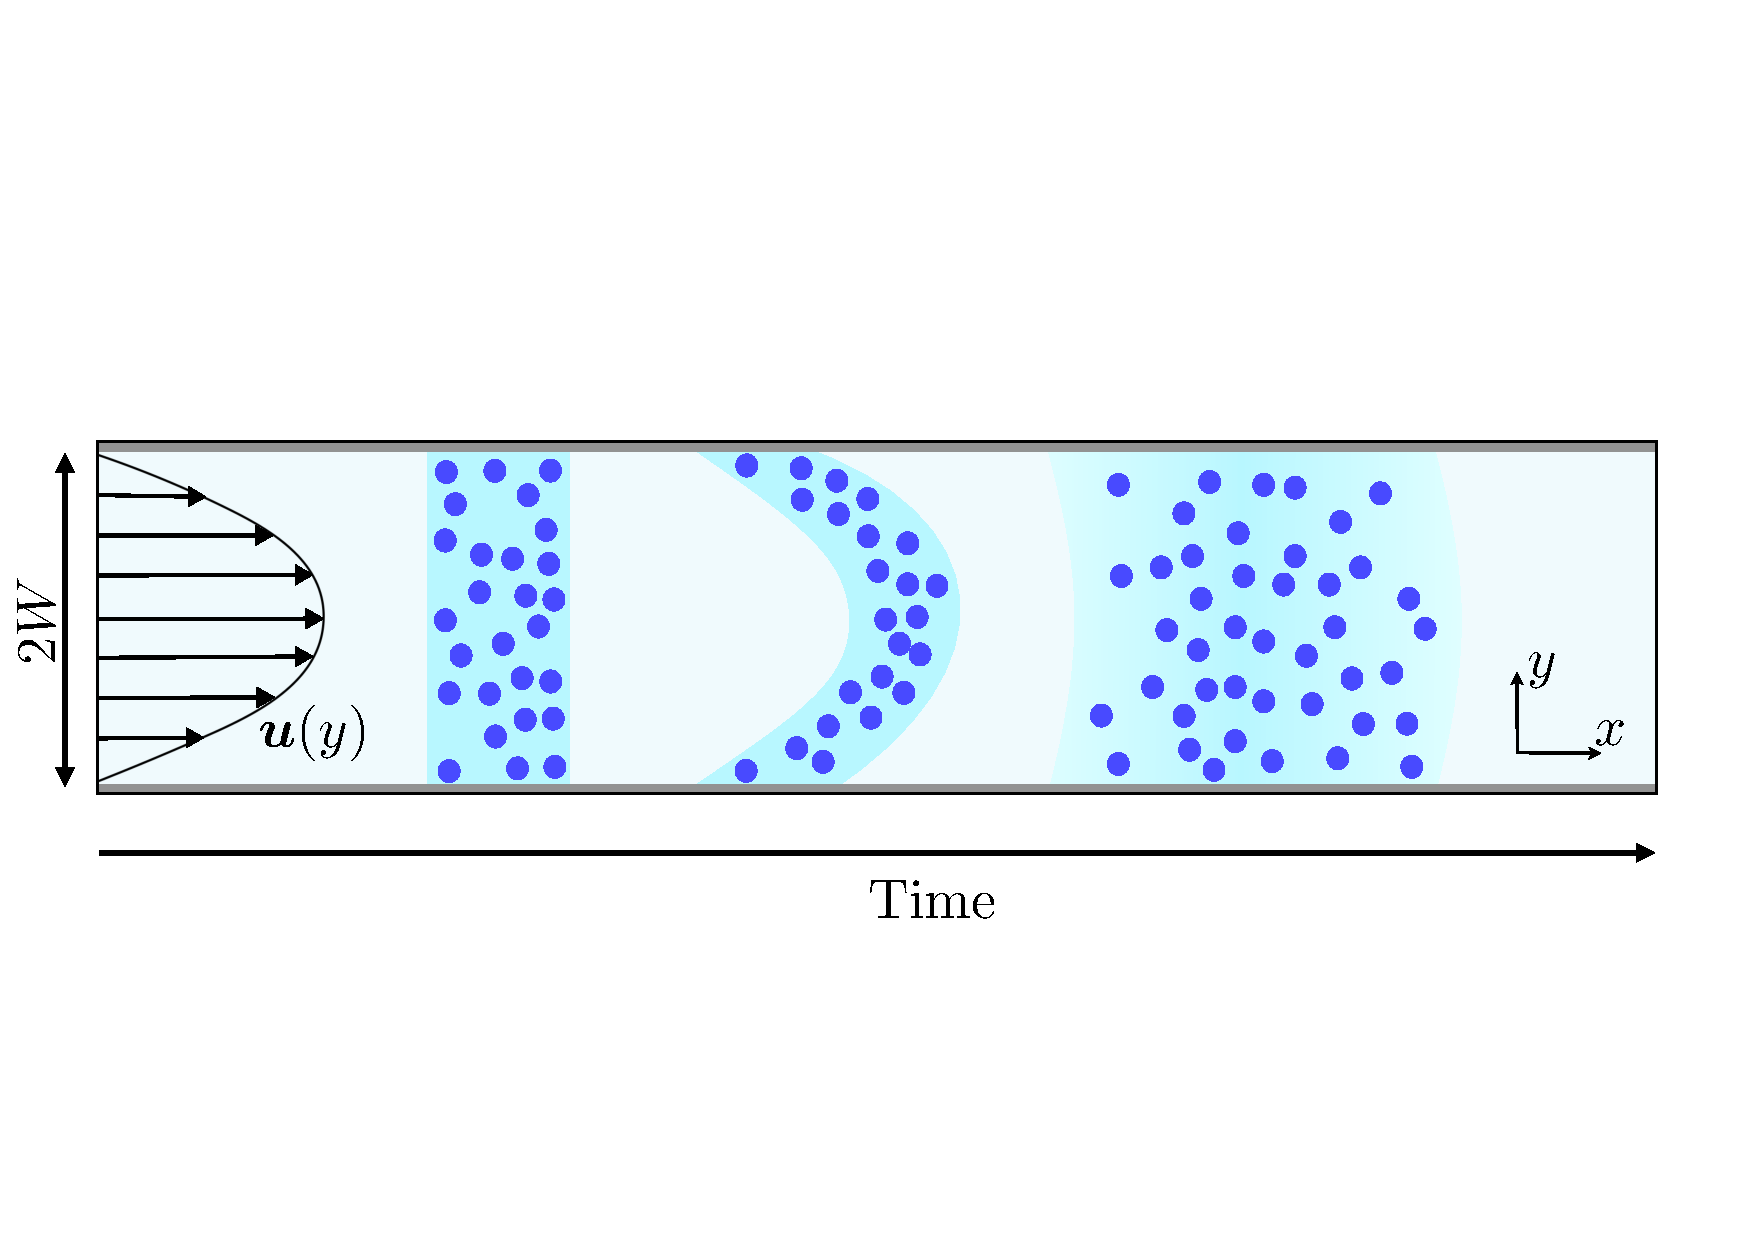
\includegraphics[width=1\textwidth]{figures/chapter4/chap4fig1.pdf}
    \caption[Schematic of the Taylor-Aris dispersion phenomenon.]{Schematic of the Taylor-Aris dispersion phenomenon. A plug of Brownian solute (darker blue) is injected in a microchannel of width $2W$. A viscous flow of velocity $u(y)$ advects the solute.}
    \label{figTaylorAris}
\end{figure}
We consider a microchannel of width $2W$ (Fig.\ref{figTaylorAris}). The fluid in that channel is advected by a unidirectional flow $u(z)\vect e_x$, where $x$ and $z$ are the direction along and normal to the channel, respectively. The flow takes a characteristic Poiseuille parabolic shape. A solute of concentration $c(x,z,t)$ and bulk diffusivity $D_0$ is injected in that microchannel. It obeys the advection-diffusion equation:
\begin{equation}
    \partial_t c + u(y)\partial_x c = D_0\left(\partial_x^2 c+\partial_y^2 c\right)~.
\end{equation}
The concentration $c$ is the sum of the cross-sectional averaged concentration $\bar c$ and a small transverse correction $c'$ induced by the shear, as:
\begin{equation}
    c(x,z,t)=\bar c(x,t)+c'(x,z,t)~,
\end{equation}
We define the transverse diffusion time $\tau_\mathrm{D}$ as:
\begin{equation}
    \tau_\mathrm{D} = \dfrac{W^2}{D_0}~.
    \label{TauD}
\end{equation}
At times larger than $\tau_\mathrm{D}$, the concentration is equilibrated across the channel width. The effective one-dimensional advection-diffusion equation reads:
\begin{equation}
    \partial_t \bar c + \bar u\,\partial_x \bar c = D_\mathrm{eff}\partial_x^2 \bar c~,
\end{equation}
where $D_\mathrm{eff}$ is an effective diffusion coefficient, called dispersion coefficient, $\bar{u}$ is the velocity average over $z$. The fluid flow velocity reads:
\begin{equation}
    u(y)=\dfrac{3}{2}\bar u\left(1-\dfrac{z^2}{W^2}\right)~,
    \qquad -W<y<W,
\end{equation}
and the dispersion coefficient is thus given by:
\begin{equation}
    D_{\mathrm{eff}} = D_0+\alpha\dfrac{\bar u^2 W^2}{D_0}~,
\end{equation}
where the $\alpha = 1/210$ in this case\footnote{The $\alpha$ coefficient is a geometrical factor, depending on the channel and flow shapes. While $\alpha=2/105$ for a Poiseuille flow in a two-dimensional channel, a cylindrical channel with a Poiseille flow had $\alpha = 1/48$, whereas a plug flow yields $\alpha = 0$.}. From there, we can identify the Péclet number $\mathrm{Pe}$, which is given by:
\begin{equation}
    \mathrm{Pe} = \dfrac{\bar u W}{D_0}~.
\end{equation}
The Péclet number compares advective to diffusive behaviour in the solute. Finally, we can write the effective diffusion coefficient (\emph{dispersion}) along the channel length:
\begin{equation}
    D_\mathrm{eff} =D_0 \left( 1+\alpha \mathrm{Pe}^2 \right)~,
    \label{Taylor-Aris}
\end{equation}
which is the classical Taylor-Aris formula ~\cite{taylor_dispersion_1953, taylor_turbulent_1954, taylor_conditions_1954, aris_dispersion_1956}. This formula provides the flow-induced enhancement of the dispersion coefficient of a solute in a channel. For $\mathrm{Pe}=0$, the dispersion should be minimal; beyond $\mathrm{Pe}^2 > 1/\alpha$, advection becomes dominant over thermal diffusion $D_0$ (Fig.~\ref{DeffD0}). It is worth noting that, while I chose to speak in terms of concentration, the above computations remain valid for the probability of presence of a single colloid in a viscous flow.
\begin{figure}
    \centering
    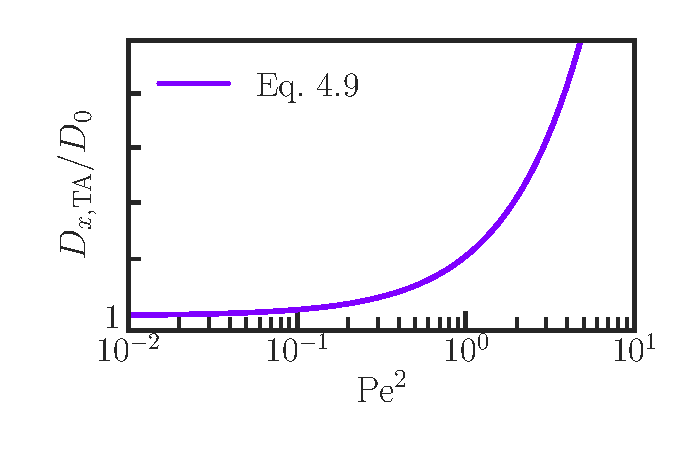
\includegraphics[width=0.8\textwidth]{figures/chapter4/DeffD0.pdf}
    \caption[Dispersion coefficient as a function of Péclet number squared according to Taylor-Aris theory.]{Predicted dispersion coefficient renormalised by the bulk diffusion coefficient $D_\mathrm{eff}/D_0$ against Péclet number squared $\mathrm{Pe}^2$ computed from Eq.~\ref{Taylor-Aris} with $\alpha = 1/48$, corresponding to the case of a cylindrical tube.}
    \label{DeffD0}
\end{figure}
Taylor-Aris dispersion is still an open field of study. Recent studies have incorporated to the original Taylor-Aris theory a range of sophistications, from time-varying flow profiles ~\cite{vedel_transient_2012, lee_taylor_2014} to particle size determination ~\cite{cottet_mixtures_2007, cottet_individual_2010, cipelletti_polydispersity_2014, lesaux_size-based_2008}, and even to active swimmers ~\cite{lagoin_enhanced_2025}, which will be the focus of the next chapter.
 
\section{Hydrodynamic interactions in an advected solute}
We present in this section a collaboration carried out with Masoodah Gunny, Alexandre Vilquin, Joshua McGraw and Blaise Delmotte, and building upon previous studies by Elodie Millan. Specifically, we wonder whether the volume fraction of a solute in a flow can influence the diffusion of this solute. This problem is highly nontrivial from an experimental standpoint. The hydrodynamic interactions between colloids, the fluid flow, and the confinement all contribute to the dynamics of the problem.  Therefore, I conduct numerical simulations to replicate the experimental results while in control of every parameter and interaction. I present here briefly our experimental protocol and the results of our collaboration. 

\subsection{Experimental setup}
This part of the chapter is largely based on Masoodah Gunny's PhD thesis manuscript ~\cite{gunny_near-surface_2025}. Experiments are carried out with silica beads of radius $a=55 \, \mathrm{nm}$ in salted water of concentration $[\mathrm{NaCl}] = 5.4-54\, \mathrm{mg.L}^{-1}$ (with corresponding Debye lengths $l_\mathrm{D} = 35-10 \, \mathrm{nm}$). The solution is injected in a microfluidic channel of length $L = 8.8\,\mathrm{cm}$, width $W = 180\,  \upmu \mathrm{ m}$ and thickness $H = 20 \, \upmu  \mathrm{m}$. A pressure gradient $\Delta P$ is then applied between the entrance and exit of the channel to start the flow. Very close to the wall, we approximate the Poiseuille profile of the flow as a linear shear $\dot s z$, with $\dot s$ a shear rate (Fig.~\ref{alex}). We take $\dot s = \Delta PH/(2\eta L)$. We are interested in the individual colloid behaviour, and thus need an imaging technique that allows for the visualisation of individual colloids rather than a global concentration profile.
\begin{figure}
    \centering
    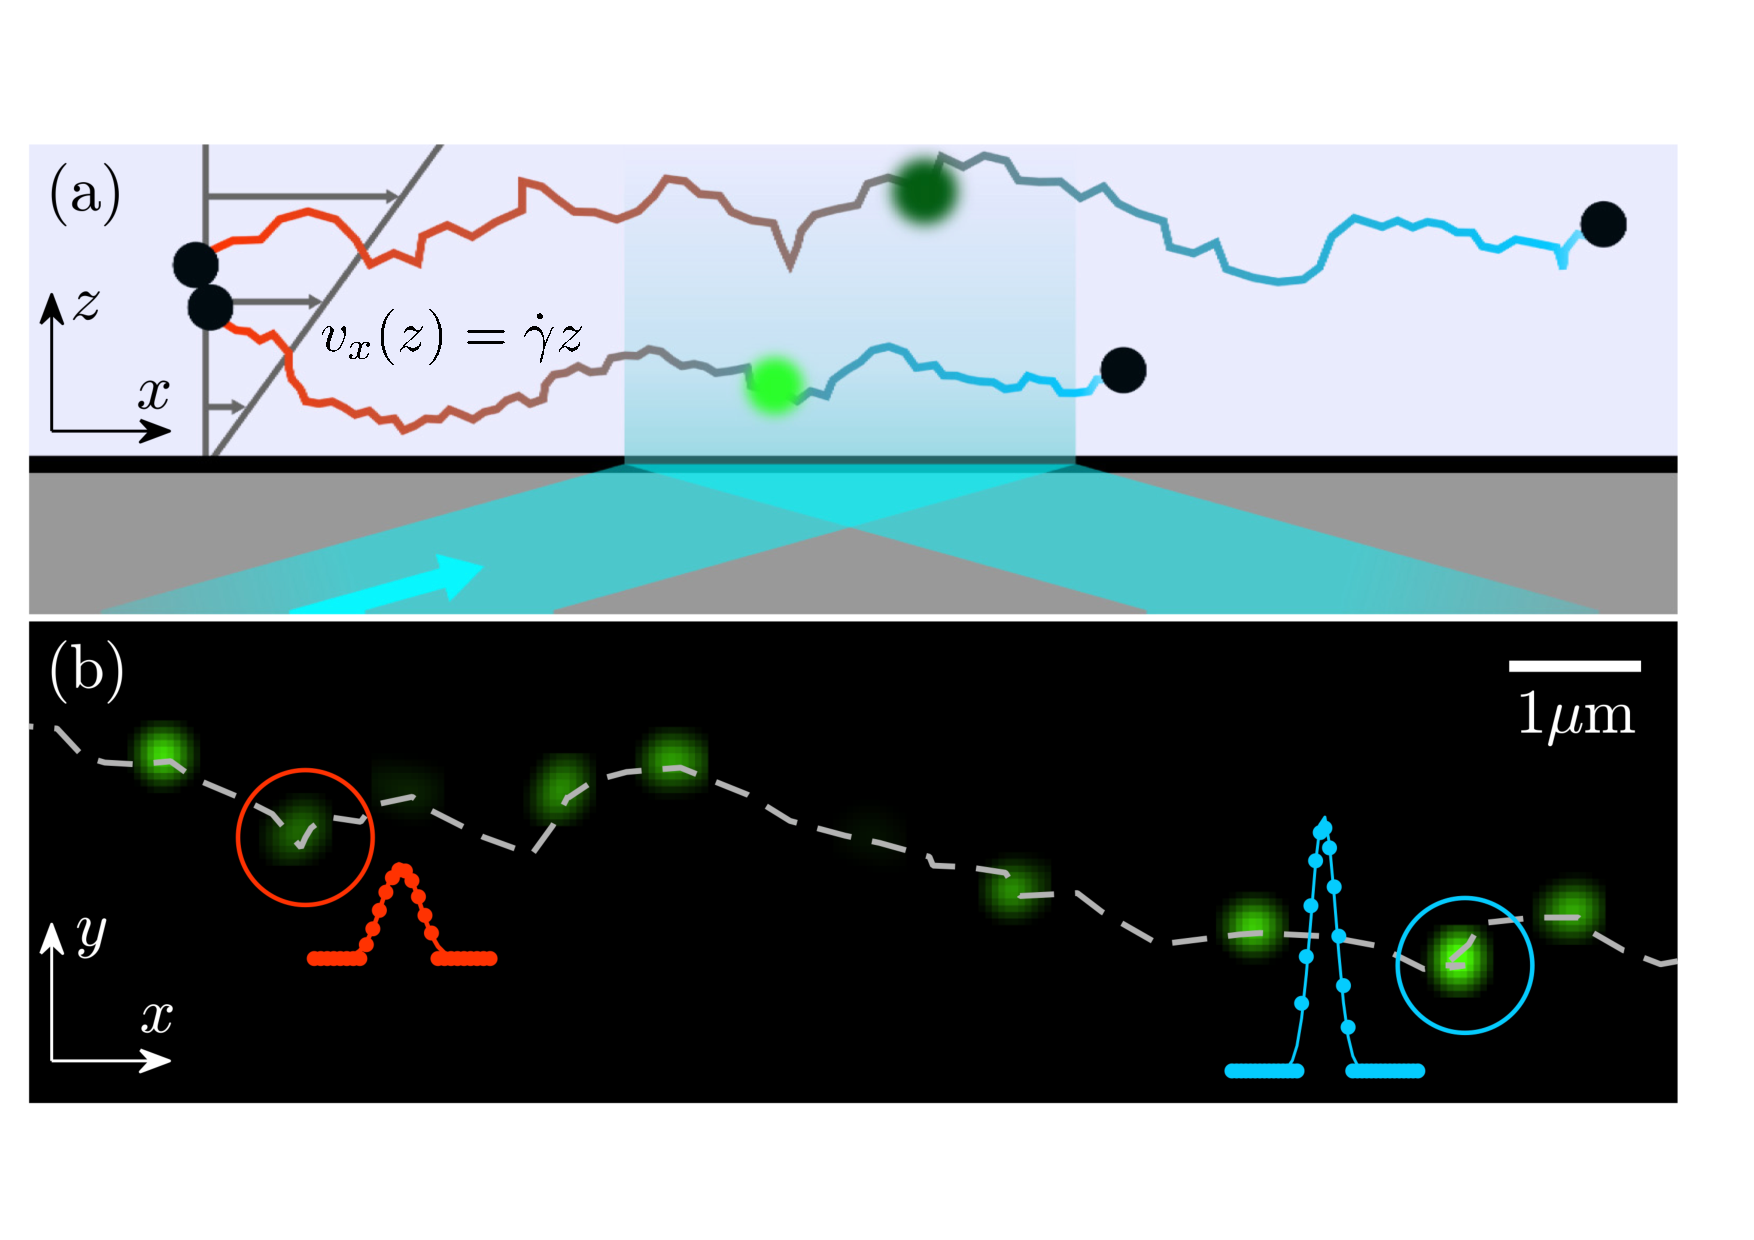
\includegraphics[width=0.9\textwidth]{figures/chapter4/alex.pdf}
    \caption[Total internal reflection fluorescence microscopy setup.]{Schematic of the Taylor-dispersion total internal reflection fluorescence microscopy setup. (a) Two colloids of radius $a=55\, \mathrm{nm}$ are advected by a shear flow of shear rate $\dot s$. As they penetrate the evanescent field, they fluoresce and their positions in all three dimensions are recovered. (b) Experimental images for a single colloid. A succession of frames taken with lag time $\tau = 12.5\, \mathrm{ms}$ is shown. Intensity profiles are represented in red and blue dots with Gaussian fits. The linked trajectory of the colloid is represented in a grey dashed line. Adapted from ~\cite{vilquin_time_2021}.}
    \label{alex}
\end{figure}
Imaging is done by Total Internal Reflection Microscopy (TIRFM) ~\cite{fish_tirf_2009} (Fig.~\ref{setup}). TIRFM has the advantage of being a sub-wavelength imaging technique which still gives information on the three coordinates of a colloid's position within the observation range. The principle of TIRFM relies on evanescence to collect information on the colloid's altitude. An incident laser beam hits the wall of the microchannel with incident angle $\theta$. This angle must obey:
\begin{equation}
    \theta > \theta_\mathrm{c}~,
\end{equation}
where $\theta_\mathrm{c}$ is the critical angle above which no refraction is permitted:
\begin{equation}
    \theta_\mathrm{c} = \sin^{-1}\left(\dfrac{n_1}{n_2}\right)~,
\end{equation}
with $n_1$ and $n_2$ the optical indices of the water solution and the solid medium, respectively, and $n_1<n_2$. Like this, refraction is prohibited, and almost all incident light is reflected. However, we know from Maxwell's equations that electromagnetic fields must remain continuous at the interface between the two media. Thus, the field must not end abruptly, but rather fade into a non-propagating electromagnetic field, which we call the evanescent wave. The penetration depth $d$ of this wave is fairly limited, at about two colloid radii, and is given by:
\begin{equation}
    d = \dfrac{\lambda_0}{4 \pi \sqrt{n_1^2 \sin^2\theta - n_2^2}}~,
\end{equation}
where $\lambda_0$ is the vacuum wavelength of the laser. This field then excites fluorescent molecules at the surface of the colloids, and we retrieve the emitted light. We can infer the distance $z$ between a colloid and the interface from the intensity a colloid emits, as:
\begin{equation}
    I(z) = I_0 \exp \left(\dfrac{-z}{d}\right)~,
\end{equation}
where $I_0$ is the maximal intensity at the interface.
\begin{figure}
    \centering
    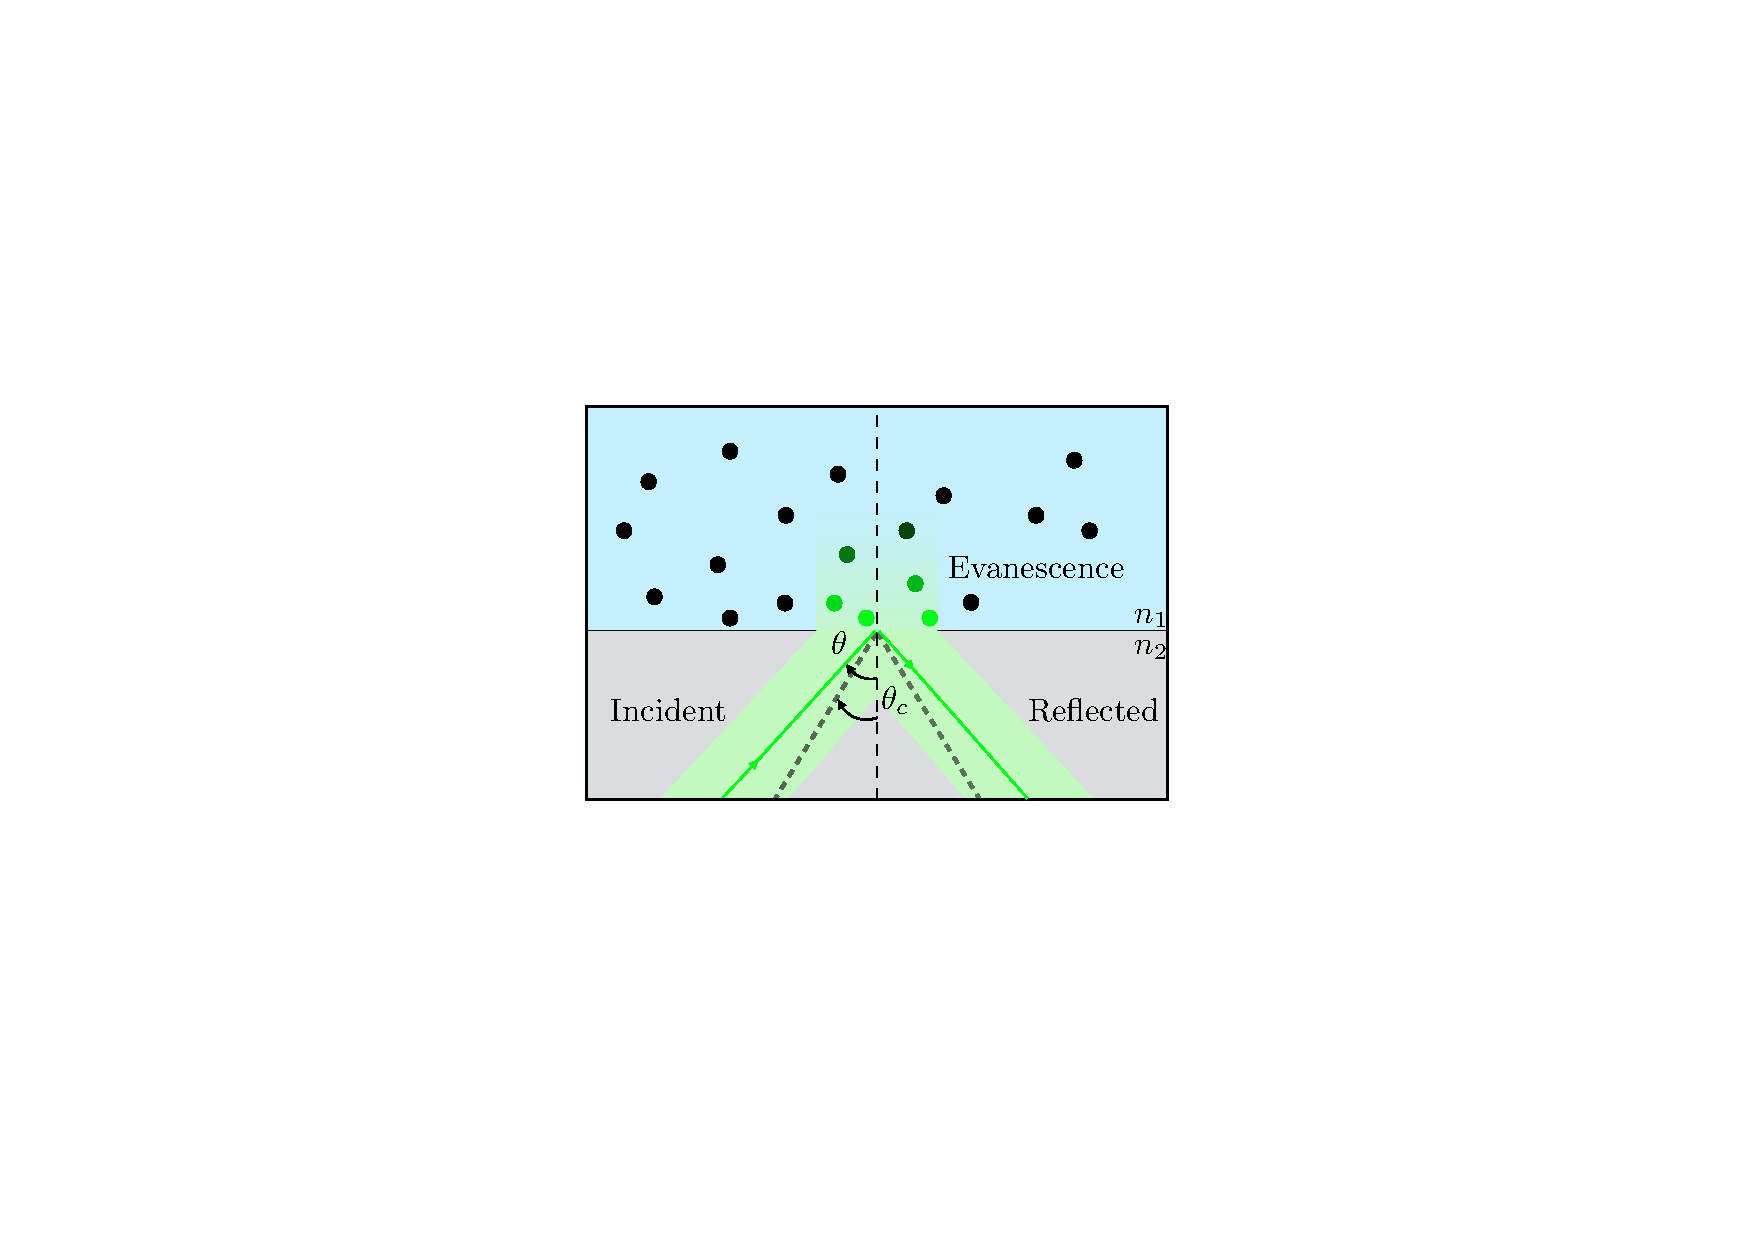
\includegraphics[width=0.6\textwidth]{figures/chapter4/setup.pdf}
    \caption[Schematic of the TIRFM evanescent wave principle.]{Principle of TIRFM. An incident beam hits the interface with an angle $\theta > \theta_\mathrm{c}$. It is almost entirely reflected back from the interface. A small portion of the beam, however, does penetrate the sample in the form of an evanescent wave. The colloids in the sample can be visualised owing to their fluorescence when they are illuminated by the evanescent wave and their altitude is then recovered from the light intensity they emit.}
    \label{setup}
\end{figure}
Snapshots of the solution under advection are taken with a camera. Trajectories are then linked from individual successive frames. From the trajectories, displacement distributions are computed, and the transverse diffusion coefficient is then defined as:
\begin{equation}
    D_y = \dfrac{\sigma_y^2}{2 \tau}~,
    \label{wrong}
\end{equation}
where $\sigma_y^2$ is the variance of the distribution of displacements in the $y$-direction, and $\tau$ is the time step between two consecutive frames, and is taken as $\tau = 1\, \mathrm{ms}$. Then, solutions of various concentrations of silica colloids in salted water are tested. It is more intelligible to speak in terms of volume fraction $\phi$, that is to say, the ratio of the volume occupied by colloids over the total volume occupied by the solution from there on. We define the volume fraction as:
\begin{equation}
    \phi = \dfrac{4 N \pi a^3}{3WLH}~,
\end{equation}
where $N$ is the total number of colloids in solution. The transverse diffusion coefficients $D_y$ computed from Eq.~\ref{wrong} are then extracted for various values of $\phi \in [5 \times 10^{-6} ; 4\times10^{-5}]$ and $\Delta P$ and shown in Fig.~\ref{nope!!!nope!!!!!!!!!}. Experimental results seem to point towards a shear rate and volume fraction dependence on $D_y$ (Fig.~\ref{nope!!!nope!!!!!!!!!}, bottom panels). Indeed, for high enough volume fractions ($\phi = 3.7 \times 10 ^{-5}$, or $0.000037\,\%$ of total volume occupied by colloids), $D_y$ becomes larger than the bulk diffusion coefficient $D_0 = 3.9\, \upmu \mathrm{m^2.s}^{-1}$, and this effect is exacerbated with higher shear rates.
\begin{figure}
    \centering
    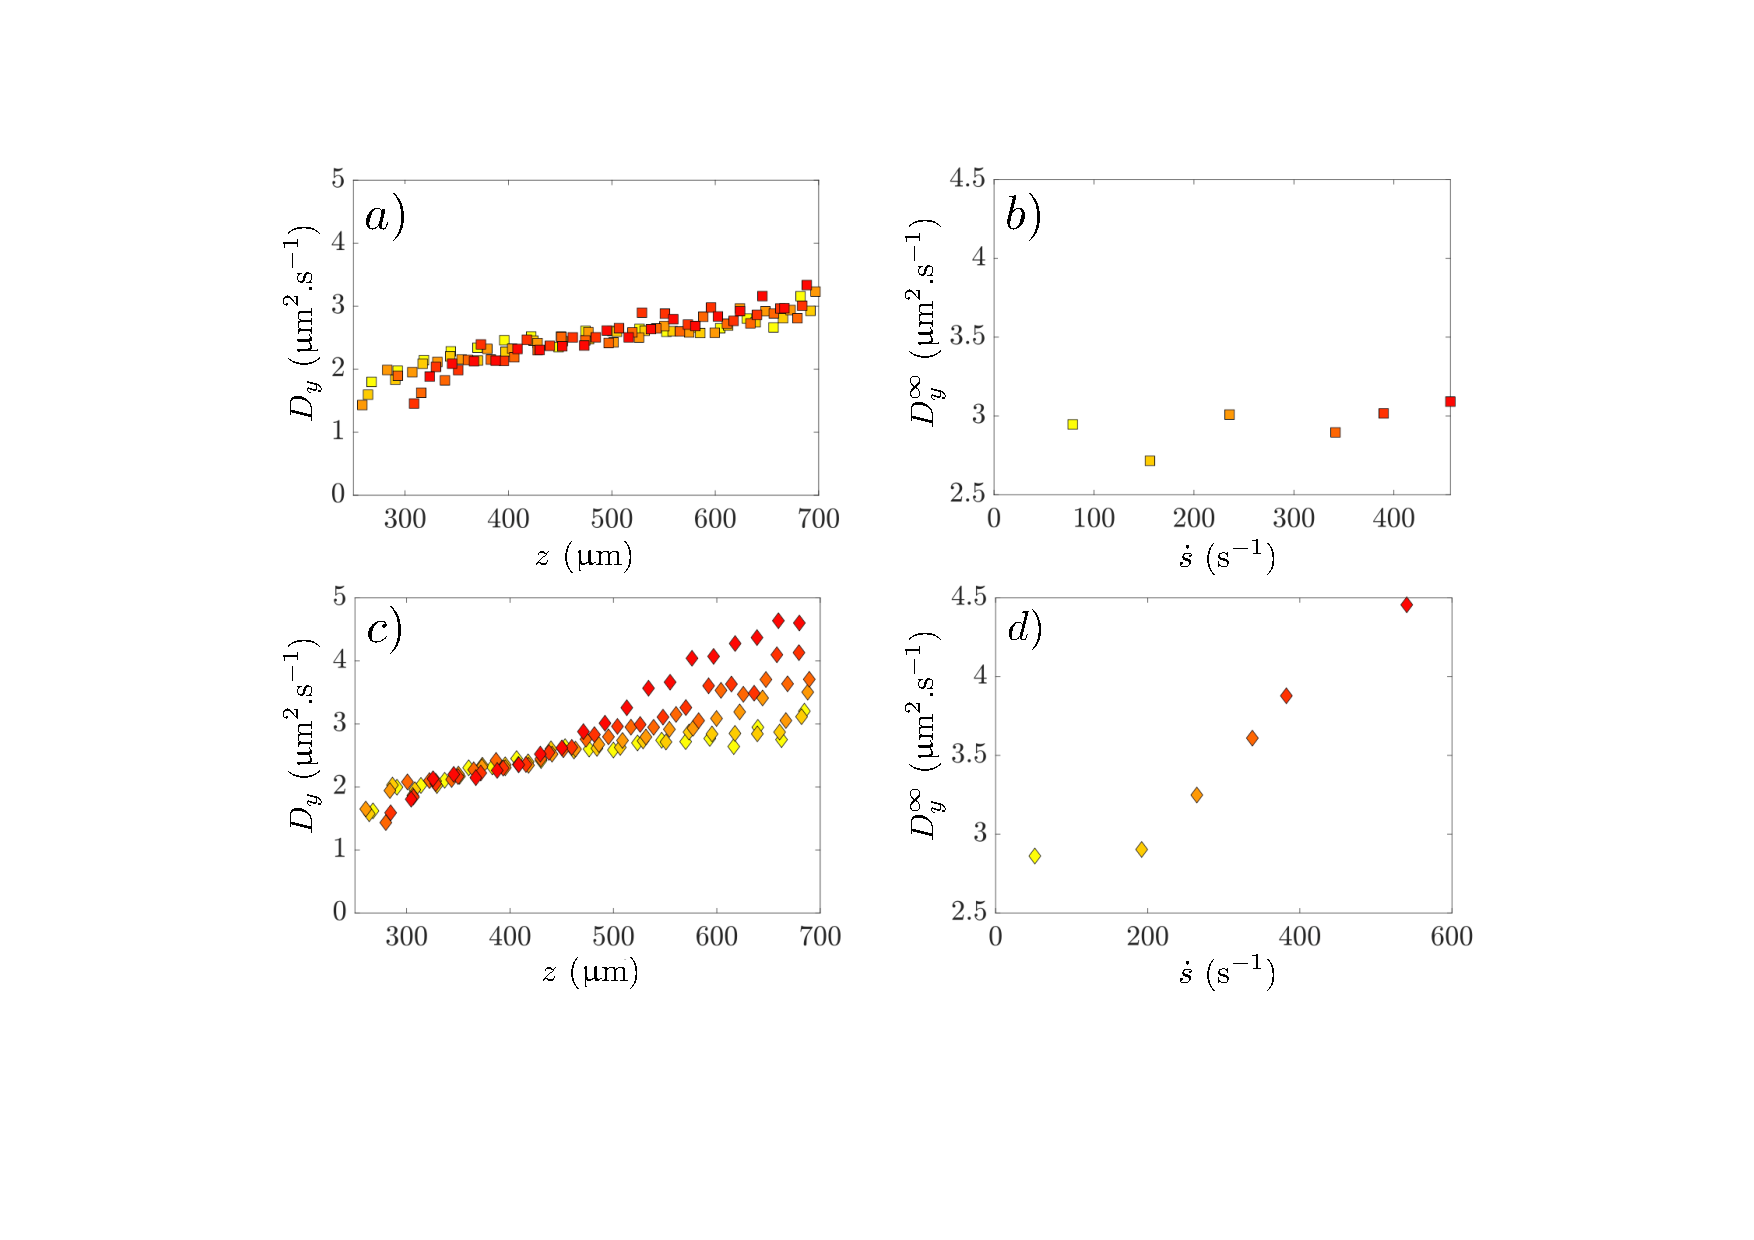
\includegraphics[width=1\textwidth]{figures/chapter4/dy_masoodah.pdf}
    \caption[Experimental results measured by TIRFM on the $y$-direction (transverse) diffusion coefficient $D_y$ for various values of shear rate $\dot s$ and volume fraction $\phi$.]{Transverse diffusion coefficients computed for $\phi =  5.4 \times 10^{-6}$ (top) and $\phi = 3.7 \times 10 ^{-5}$ (bottom) and for various pressure gradients $\Delta P$ or equivalent shear rates $\dot s$ (in colours). Left panels show the diffusion at binned heights $z$ above the channel wall. The bulk diffusion coefficient $D_0 = 3.9 \,  \upmu \mathrm{m}^2.\mathrm{s}^{-1}$ is shown in horizontal dashed lines. Adapted from ~\cite{gunny_near-surface_2025}.}
    \label{nope!!!nope!!!!!!!!!}
\end{figure}
There are a few potential causes that can easily be ruled out by carrying out numerical simulations. This has already been done by Élodie Millan for the case of electrostatic interactions. We now explore the role of hydrodynamic interactions between the colloids to understand their role in this experimental observation.

\subsection{Numerical methods}
As our collaborators in ESPCI hypothesised a hydrodynamic effect causing the enhancement in transverse diffusion $D_y$, I conduct all the forthcoming simulations using the RigidBlobWalls ~\cite{sprinkle_driven_2020}. This package, described more in depth in chapter~\ref{chapter2}, is optimised for the simulation of colloids in hydrodynamic and electrostatic interactions, and allows boundary interactions and shear flows. The task involves reproducing the TIRFM setup numerically, generating trajectories in the same conditions as the experiments, and extract similar quantities from these trajectories. The point is to obtain data from a perfectly controlled environment, with perfect tracking of every colloid's position, and with all interactions known. 
\begin{figure}
    \centering
    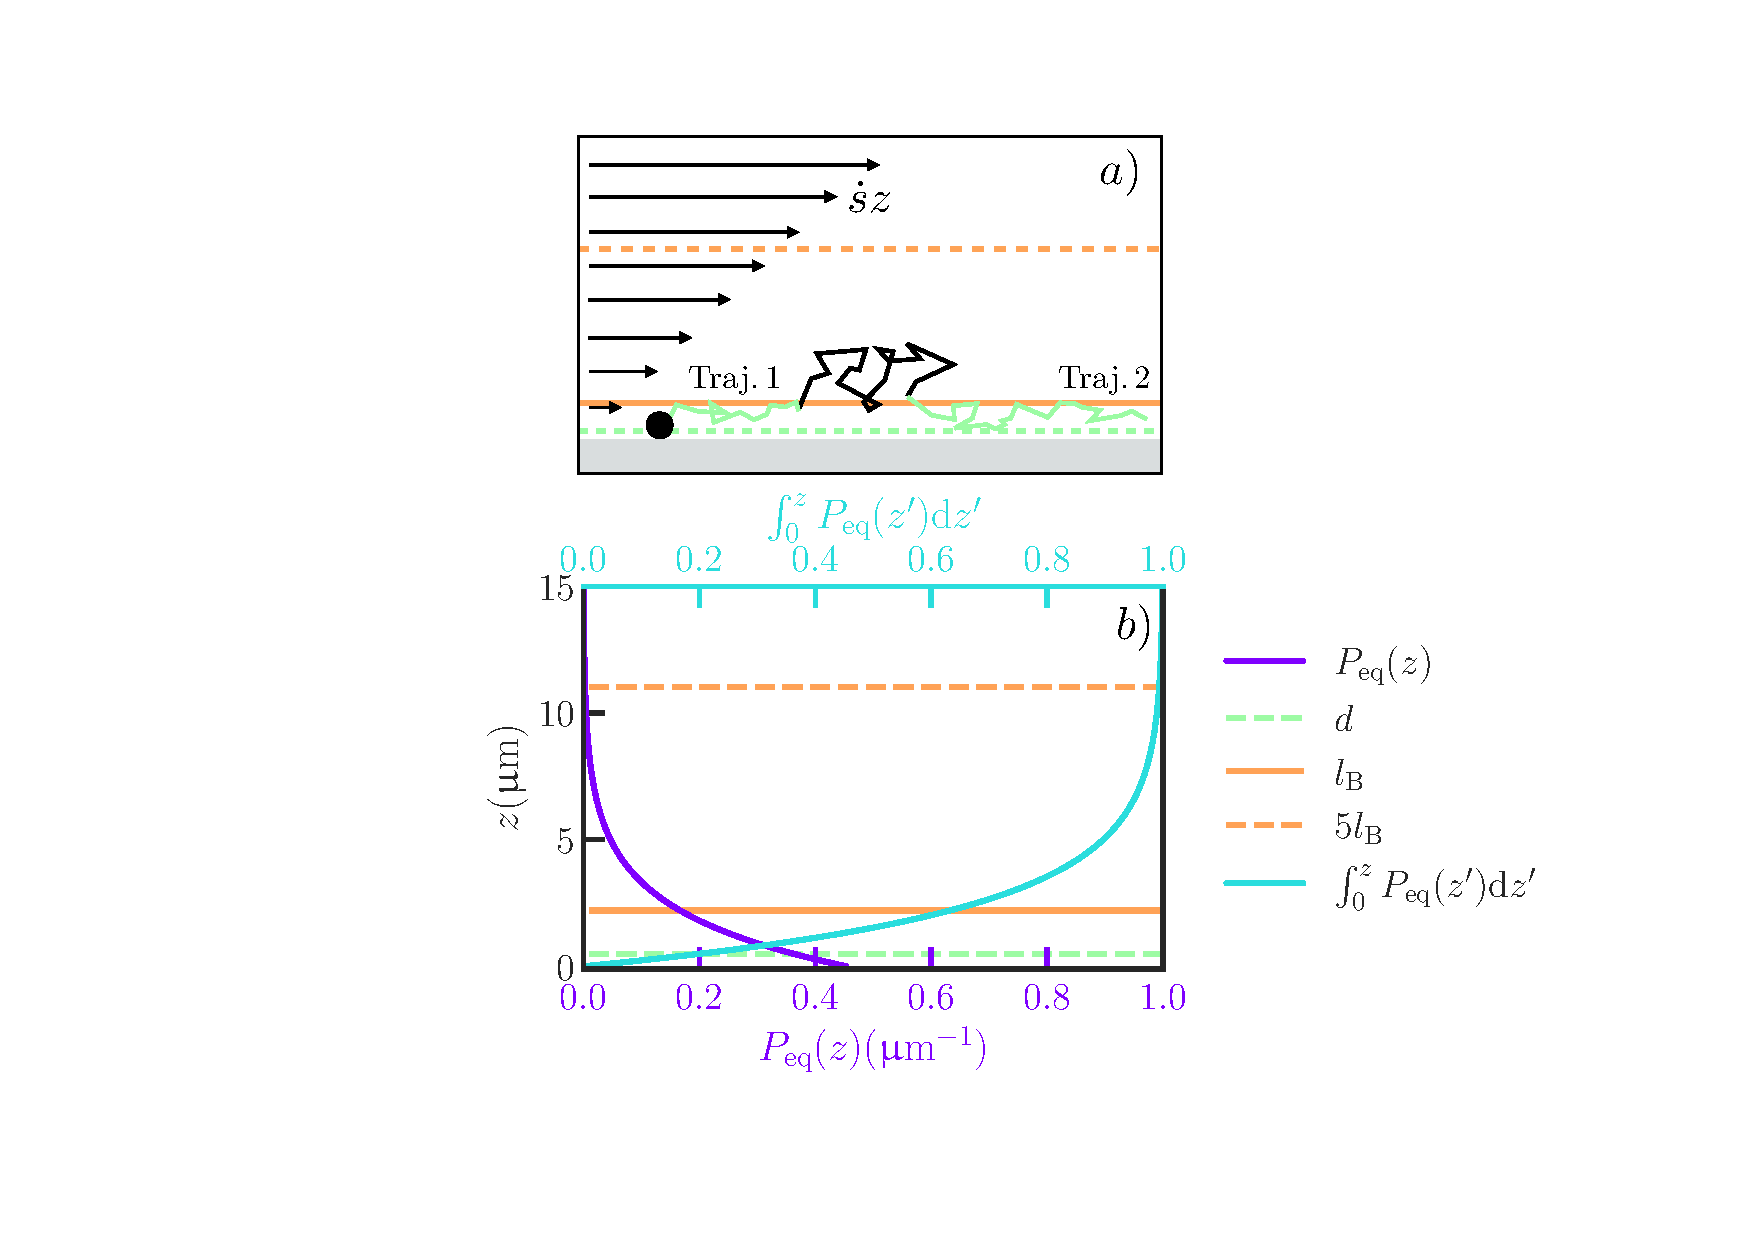
\includegraphics[width=1\textwidth]{figures/chapter4/numerical_setup.pdf}
    \caption[Numerical simulation setup mimicking TIRFM results.]{Numerical simulation setup. $a)$ Colloids are initialised in position in a box of dimensions $L_x \times L_y \times 5 l_\mathrm{B}$, with $l_\mathrm{B}$ the Boltzmann length. The box is periodic in the $x-$ and $y-$ directions, with a no-slip boundary at $z=0$. A shear flow of shear rate $\dot s$ is applied in the $x$ direction. Trajectories are recorded for a total time of $T = n_\mathrm{steps} \times \Delta t$, where $n_\mathrm{steps}$ is the total number of simulated steps, and $\Delta t$ is the duration of one time step. Trajectories crossing the evanescent limit $d$ are killed, and trajectories re-entering below $d$ are tracked as new trajectories if they exist for more than three time steps. $b)$ Equilibrium distribution of colloids in solution, as predicted by the Gibbs-Boltzmann distribution (blue, Eq.~\ref{GBch4}) and corresponding cumulative sum (red, Eq.~\ref{eq:cumsum}). The evanescent limit $d$ is represented in green. The Boltzmann length $l_\mathrm{B}$ is represented with a yellow line. We estimate that $99\,\%$ of the colloids lie under $5l_\mathrm{B}$ (yellow dashed line). }
    \label{numerical_setup}
\end{figure}

Simply put, a simulation has four main steps:
\textbf{Parametrisation.} The user provides the physical parameters (buoyant mass of a colloid $\Delta m$, colloid radius $a$, shear rate $\dot s$, fluid viscosity $\eta$, thermal energy $k_\mathrm{B}\Theta$, Debye length $l_\mathrm{D}$, amplitude $A$ of the electrostatic repulsion potential, evanescent limit $d$) and simulation parameters (time step $\Delta t$, total number of steps $n_\mathrm{steps}$, periodic lengths $L_x$ and $L_y$). This is done using the \texttt{inputfile.dat} and \texttt{parameters.py} scripts. The \texttt{parameters.py} script then reads \texttt{inputfile.dat} to convert, calculate, and pass parameters to the other scripts. As we discussed in the previous paragraphs, the two key quantities we must have full control over are the shear rate $\dot s$ and the volume fraction $\phi$. The former is simply given as an input to the code in \texttt{inputfile.dat}, whereas the latter must be entered indirectly in the form of the total number $N$ of \emph{blobs}, which in this case are equivalent to colloids. 
\textbf{Initialisation.} \texttt{sample\_initial\_positions\_gb.py} reads from \texttt{parameters.py} the array of $\phi$ values to be probed. 
The volume fraction is actually ill-defined in our system if considered without care. Indeed, the simulation code is built to either work in triply periodic boundaries, or doubly periodic in $(x, y)$ and half-infinite in $z$ with a confining plane at $z=0$. This means the maximum height above which colloids do not escape is set physically, not through user input directly. We can only decide the initial positions of the colloids, but without proper care once the system reaches equilibrium, colloids diffuse in the vertical direction to preferential positions. We recall from Chapter 3 that the distribution of the positions in the grand-canonical ensemble is predicted from the Gibbs-Boltzmann distribution:
\begin{equation}
    P(z) = \dfrac{1}{Z} \exp \left( \dfrac{U(z)}{k_\mathrm{B}\Theta} \right)~,
    \label{GBch4}
\end{equation}
with $1/Z$ the partition function, and $U(z)$ the total potential energy, given here by:
\begin{equation}
    \dfrac{U(z)}{k_\mathrm{B}\Theta} = A \exp\left(- \dfrac{z}{l_\mathrm{D}}\right) + \dfrac{z}{l_\mathrm{B}}~,
\end{equation}
with $A$ the dimensionless magnitude of the electrostatic repulsion potential. The distribution of colloid positions along $z$ can be integrated, as:
\begin{equation}
\int_{0}^{z} P_\mathrm{eq}(z')\, \mathrm dz'~,
\label{eq:cumsum}
\end{equation}
to show that about $99\,\%$ of the colloids lie under $5l_\mathrm{B}$, and about $60\,\%$ below $l_\mathrm{B}$ (Fig.~\ref{numerical_setup}b)). 

Under these conditions, two problems emerge: first, if we choose to lower the simulation cost by using a small box of height $H_\mathrm{box}$ with $H_\mathrm{box}<5l_\mathrm{B}$ to place our colloids at the beginning of the simulations, the solution will inevitably homogenize to a lower volume fraction after some simulation time (Fig.~\ref{badlB}). Secondly, one cannot simply choose a volume fraction for the whole box and homogeneously place the colloids in that box. Colloids diffuse in the vertical direction and reach the Gibbs-Boltzmann distribution, which is not homogeneous (Fig.~\ref{numerical_setup} b)). Thus, the volume fraction is higher close to the wall and lower far from it (Fig.~\ref{numerical_setup} b)). To compute the volume fraction $\phi_{5l_\mathrm{B}}$ for the whole $5l_\mathrm{B}$ slab in order to retrieve the target $\phi$ within the $d$ slab, we use:
\begin{equation}
    \phi_{5l_\mathrm{B}} = \dfrac{\phi \lambda_\mathrm{e}}{5l_\mathrm{B} \dfrac{1}{Z}\int_0^{\lambda_\mathrm{e}} P_\mathrm{eq}(z) \mathrm{d}z }~.
\end{equation}
Then, we simulate the whole $5l_\mathrm{B}$ slab and fill it with the adequate amount of colloids to reach the desired $\phi$. Given that, for our system, $5l_\mathrm{B} = 5.5 \times 10 ^{-2} \, \mathrm{m}$, and the TIRFM observation window is of $22 \, \upmu \mathrm{m} \times 22 \, \upmu \mathrm{m}$, we estimate the total amount of blobs in a simulation $N = 3.7\times 10^{7}$ to reach a target volume fraction $\phi = 4 \times 10^{-4}$. This number is clearly high and expensive to simulate; we must find a workaround. A simple way of doing so is to artificially lower $l_\mathrm{B}$. By taking a much higher value for the gravitational acceleration, at $g^* = 5000 \times g$, the new Boltzmann constant is $l_\mathrm{B}^* = 2.20 \times 10^{-6} \,\mathrm{m}$, which in turn gives a simulation of $N = 152$ colloids. This is much more reasonable.
\begin{figure}
    \centering
    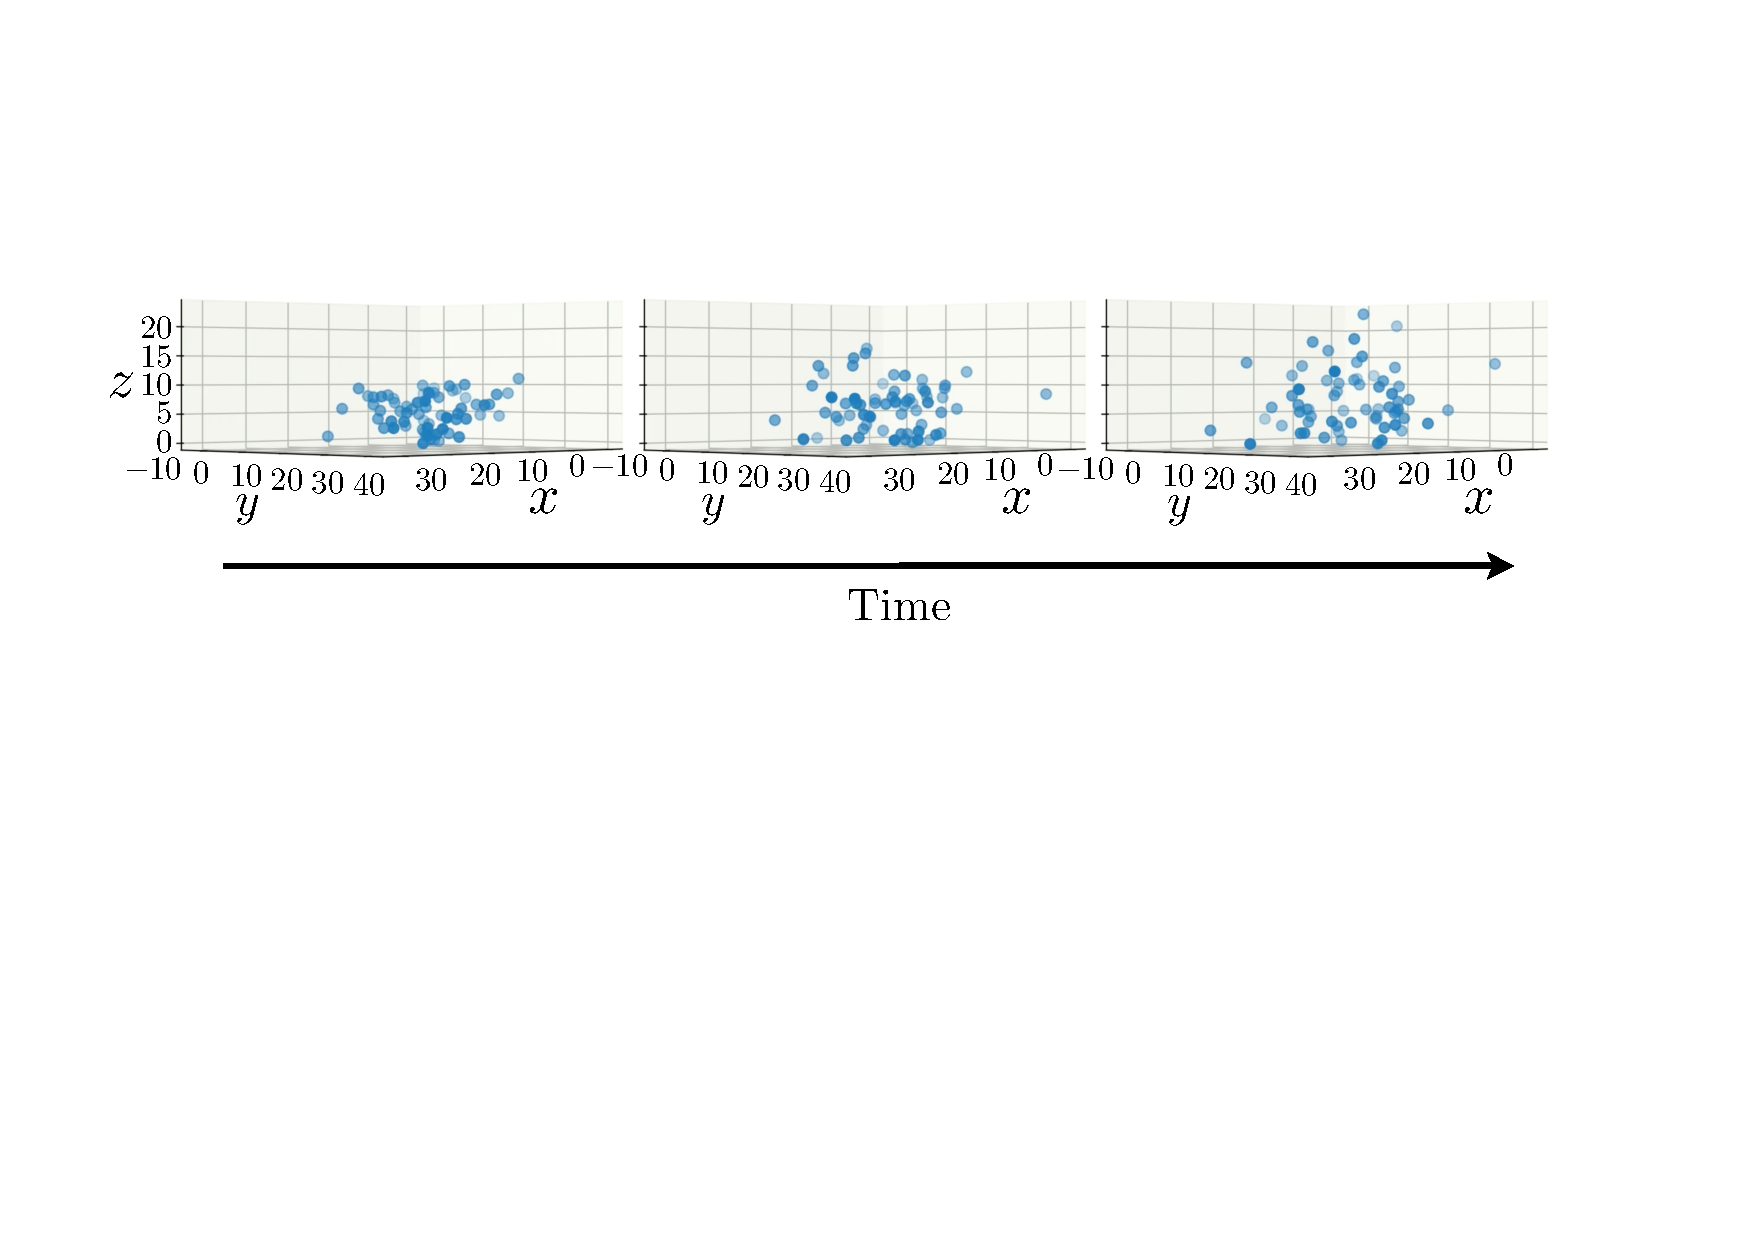
\includegraphics[width=1\textwidth]{figures/chapter4/badlB.pdf}
    \caption[Wrong initialisation of the system.]{Numerical simulation results at initialisation and through time, for a bad initialisation of the system. Colloids were laced in a $10\,\upmu \mathrm{m}$  tall box and left to thermalise with a Boltzmann length of $l_\mathrm{B} = 1.1 \times 10 ^{-2} \, \mathrm{m}$.}
    \label{badlB}
\end{figure}

\texttt{sample\_initial\_positions\_gb.py} creates, in the current working directory, a new directory for each value of $\phi$. In each new directory, it writes all the simulation scripts. Finally, and most importantly, it computes the initial colloid positions within the simulation box from the Gibbs-Boltzmann distribution of Eq.~\ref{GBch4} using a simple exclusion algorithm, and writes them to \texttt{sphere\_array.clones}. This step is crucial to ensure that the system is prethermalised, and avoids a potentially costly prethermalisation step. This script can also be used to verify that the Gibbs-Boltzmann distribution is respected and that the system is properly thermalised.
\textbf{Simulation.} The script \texttt{multi\_bodies.py} calls the entire simulation pipeline and launches the shear flow on the pre-thermalised colloidal suspension. It writes the trajectories at each time step to \texttt{run\_blobs.sphere\_array.config}. Other relevant simulation data, such as failed iterations and total computation time, are written to auxiliary output files.
\textbf{Data treatment.} From the trajectories stored in \texttt{run\_blobs.sphere\_array.config}, the trajectories are parsed, and the particle displacements are computed. We limit our studies to the same field of view as experiments. This means that we must kill in the treatment process the trajectories escaping $d$. Furthermore, if they re-enter the field of view for long enough time durations (we choose three consecutive time steps), their trajectories are treated as new trajectories by the treatment code. MSDs are computed from displacements on each trajectory and then binned by average height. Diffusion quantities are then extracted from the MSD if, and only if, a diffusive regime is identified, namely beyond the transverse diffusion time $\tau_\mathrm{D}$ and when the log-log fits yield a time exponent equal to 1.

\subsection{Results}
Finally, we can compare the results of the simulations to the experimental results. We compute the normalised transverse diffusion coefficient $D_y/D_0$ as a function of the average trajectory height for various values of $\phi$ and $\dot s$ (Fig.~\ref{Dycolormap}). We notice that, in contrast to the experimental results, no clear dependence of $D_y$ on $\phi$ or $\dot s$ is visible. The overall tendency of $D_y/D_0$ shows a slight increase the further from the contact with the wall, and quickly reaches a saturation around 1. This is in agreement with the expected behaviour of a Brownian solute in a viscous fluid, and with Brenner~\cite{brenner_slow_1961} and Faxen's~\cite{Faxen_1924}laws. The absence of any clear dependence on $\phi$ and $\dot s$ suggests that the experimental results may be due to an artefact, and that the observed enhancement of $D_y$ may not be due to hydrodynamic interactions. This is in line with the fact that, at such low volume fractions, hydrodynamic interactions should be negligible. However, it is worth noting that experiments and numerical data were treated differently. Indeed, in experiments, trajectories were first linked from different frames, and displacements were computed from these trajectories. In simulations, we directly access the whole labeled trajectories, thus ruling out any potential tracking artifact. It is worth noting that the diffusion coefficient $D_y$ itself has different definitions between our simulation results and the experiments. In experiments, $D_y$ is computed from the variance of the distribution of displacements in the $y$-direction at a fixed time step $\tau$, as shown in Eq.~\ref{wrong}. If the system is not in a diffusive regime, the extracted coefficient may not be meaningful. From numerically generated data, we compute $D_y$ from the slope of the MSD in the diffusive regime.
\begin{figure}
    \centering
    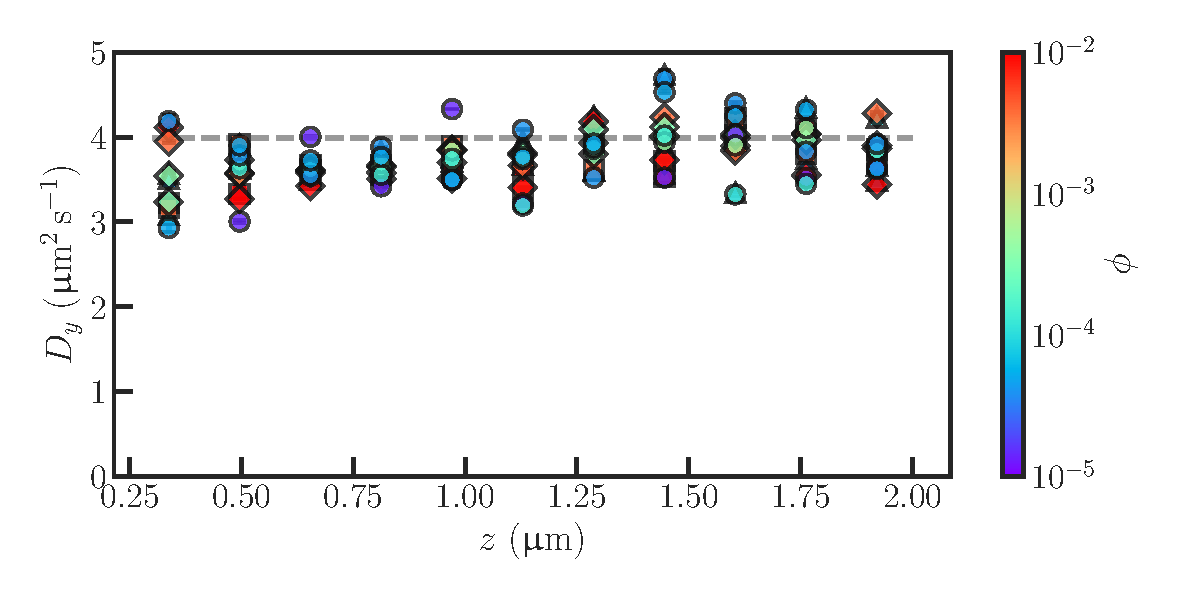
\includegraphics[width=1\textwidth]{figures/chapter4/Dyfz_colormap.pdf}
    \caption[Numerical results on the transverse diffusion coefficient $D_y$ for various values of shear rate $\dot s$ and volume fraction $\phi$.]{Normalised transverse diffusion coefficient $D_y/D_0$ as a function of average trajectory heights. Simulations were run once for each $(\phi, \dot s)$ couple and for $N_\mathrm{steps} = 50000$, with time step $\Delta t = 0.0001\, \mathrm{s}$, fluid viscosity $\eta = 0.001 \, \mathrm{Pa.s}$, colloid radius $a = 55 \, \mathrm{nm}$,  buoyant mass $\Delta m = 1.92 \times 10^{-16}\, \mathrm{kg}$, gravity acceleration $g = 5000 \times 9.81\, \mathrm{N.m}^{-2}$, thermal energy $k_\mathrm{B}\Theta = 4.14 \times 10 ^{-21}\, \mathrm{J}$, and $d = 1800 \, \mathrm{nm}$.  The colormap represents volume fractions. Disks correspond to shear rate $\dot s = 100.0 \, \mathrm{s}^{-1}$, squares to $\dot s = 500.0\, \mathrm{s}^{-1}$, triangles to $\dot s = 600.0\, \mathrm{s}^{-1}$ and diamonds to $\dot s = 1000.0\, \mathrm{s}^{-1}$. }
    \label{Dycolormap}
\end{figure}
Investigations are still being conducted to understand the origin of this discrepancy. We are currently analysing numerically generated TIRFM-like videos, with the same tracking and data analyses as the experiments used. If the effect then becomes visible, it would point towards a numerical artefact in the data extraction. However, if the effect is not visible, more investigations would be needed. We could for instance verify the actual volume fractions in experiments to fully rule out hydrodynamic effects.

\section{Take-home message}
In this chapter, we introduced the Taylor-Aris dispersion theory for Brownian solute in viscous fluid flows. We established that, in a Poiseuille flow, fluctuations permit a broadening of the concentration profile in time. This theory was the framework for our collaboration with Masoodah Gunny, Joshua McGraw, Blaise Delmotte and Alexandre Vilquin. We numerically replicated their experimental setup, consisting of a Poiseuille flow advecting a Brownian solute in a rectangular microchannel. We measured the transverse diffusion coefficient, orthogonal to the flow direction. We observed no notable effect on this coefficient from the fluid velocity or the volume fraction of the solute. We concluded that, although our simulations seem not to indicate an effect of hydrodynamic interaction between colloids on the dispersion coefficient, a new treatment should be carried out both on the numerically generated and experimental data, using exactly the same protocol. This would thus definitely rule our either hydrodynamic effects, or treatment artifacts. 

This chapter also served as in introduction to chapter 5, where we investigate the Taylor-Aris dispersion of an active solute.